% Persian title page partial for Pandoc / Quarto
\usepackage{graphicx}
\usepackage{etoolbox}

\makeatletter
\def\maketitle{%
  \begin{titlepage}%
    \centering
    \vspace*{1.5cm}
    $if(title)${\Huge\textbf{$title$}\par}$endif$
    \vspace{0.8em}
    $if(subtitle)${\large $subtitle$\par}$endif$
    \vspace{1.2cm}
    \ifdefined\includegraphics
      \IfFileExists{images/cover.png}{%
        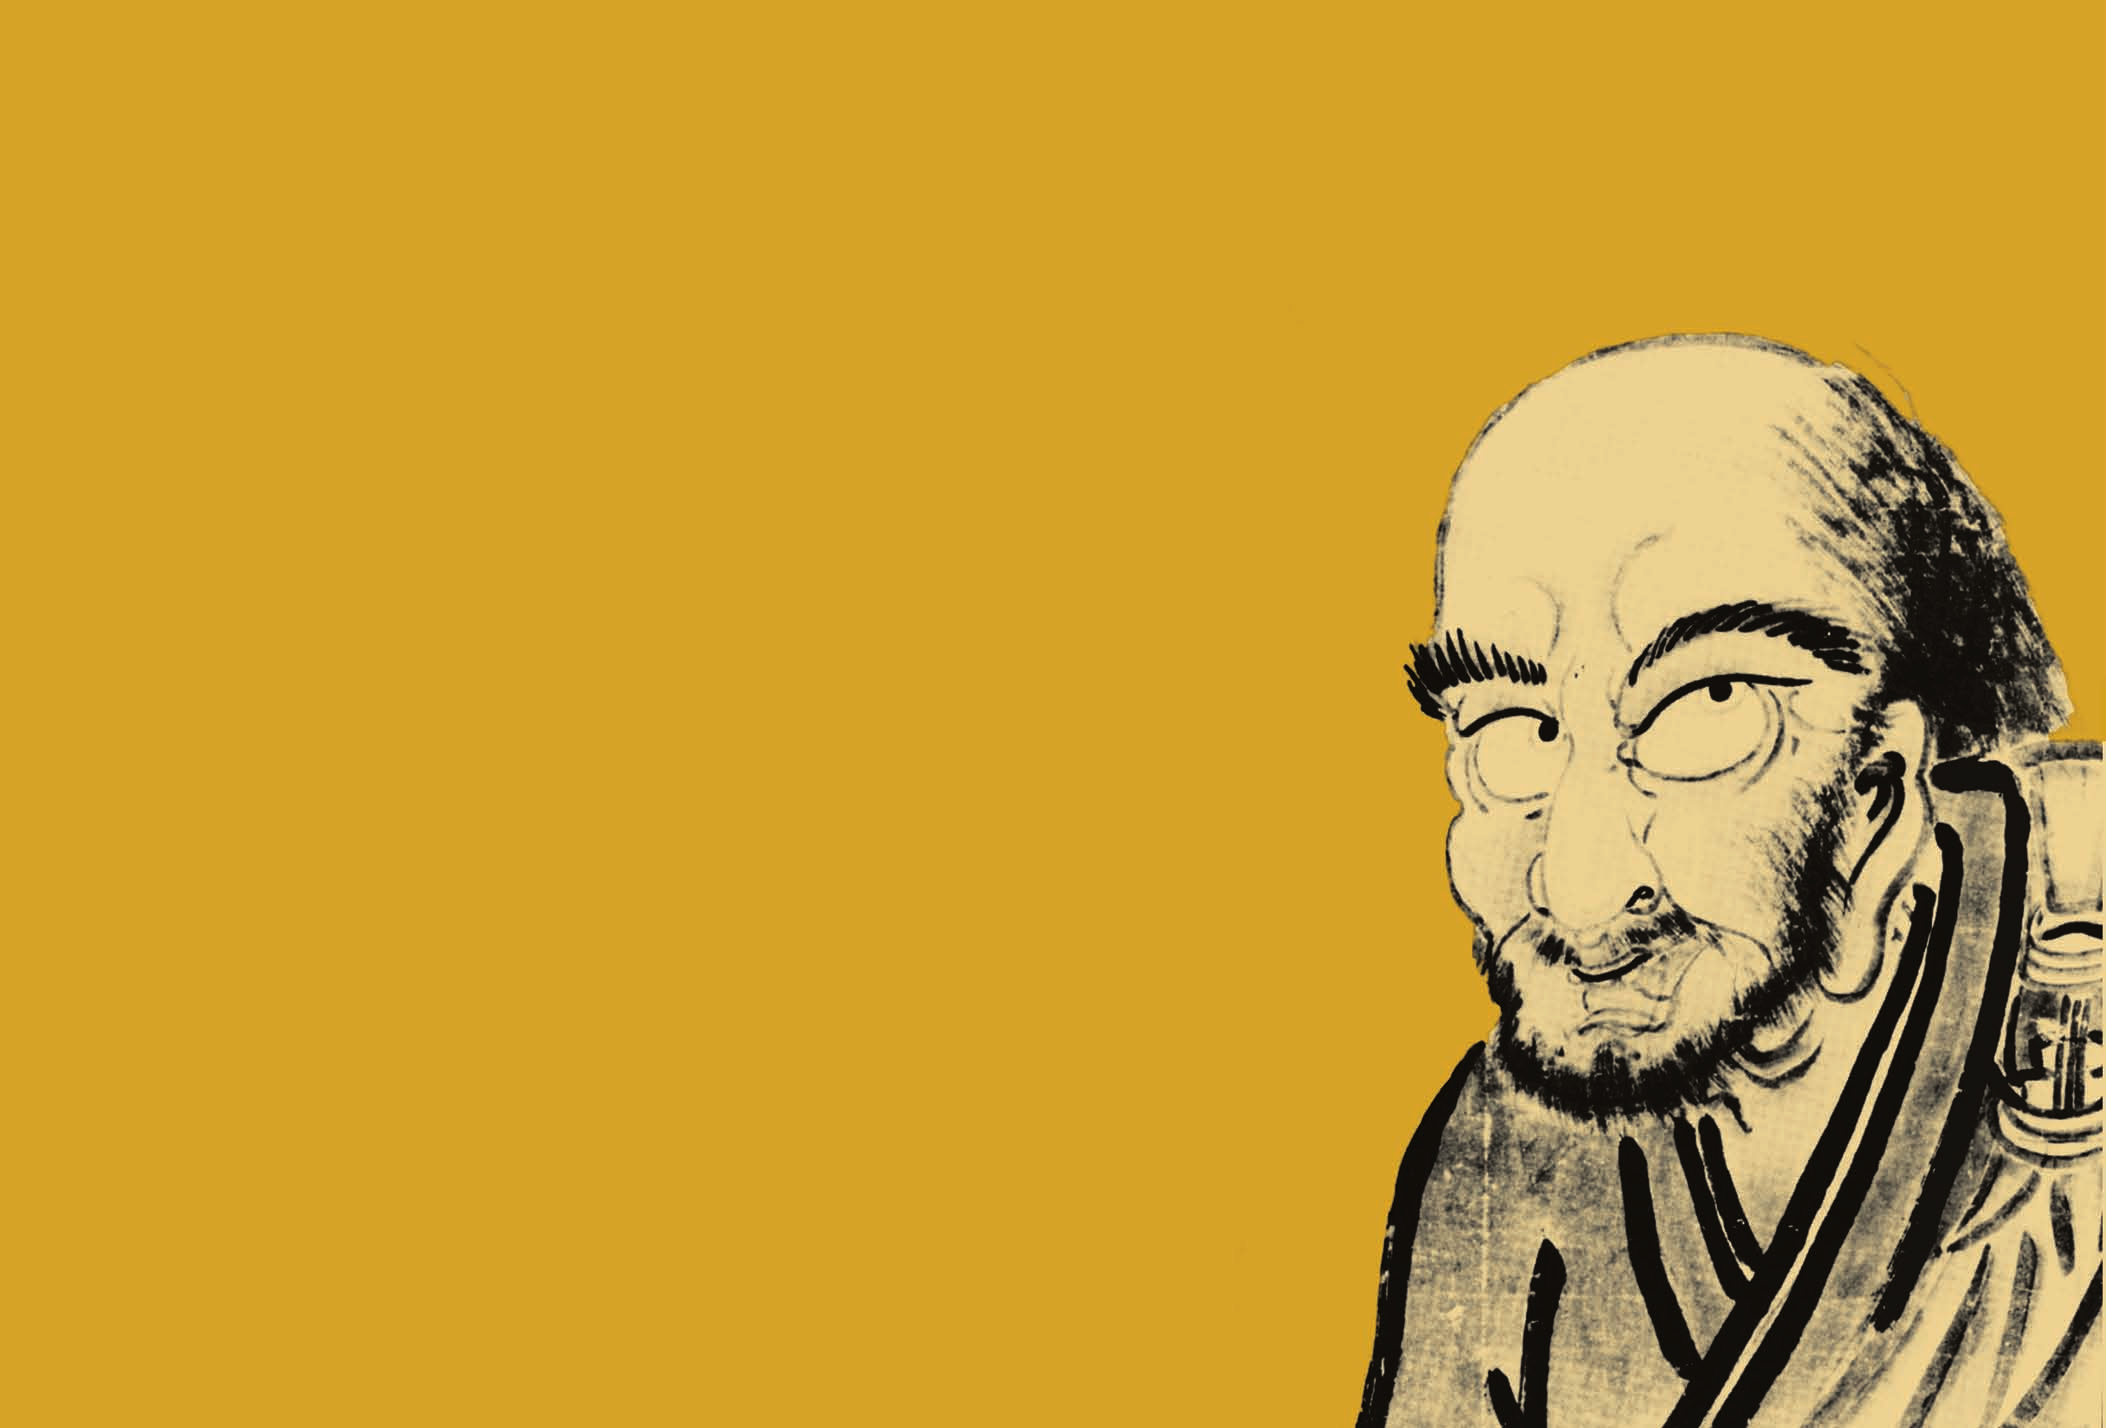
\includegraphics[width=0.32\textwidth]{images/cover.png}\par
      }{}%
    \fi
    \vspace{1.5cm}
    {\normalsize
      گفتارهای استاد چَن: \textbf{لین‌جی هوی‌جائو}\par
      گردآورنده: \textbf{هوی‌ران از سان‌شِنگ}\\[1.2em]
      ترجمهٔ انگلیسی و شرح: \textbf{روث فولر ساساکی}\par
      با همکاری: \textbf{یاناگیدا سیزان} و \textbf{ایرییا یوشی‌تاکا}\par
      ویراستهٔ: \textbf{توماس یوهو کرشنر}\\[1.2em]
      برگردان به فارسی: \textbf{$for(authors)$$it.name.literal$$sep$ \and $endfor$}\par
    }
    \vfill
    {\small
      مؤسسهٔ نانزان برای دین و فرهنگ\\[0.5em]
      $if(book-version)$$book-version$\quad•\quad$endif$$book-date$\par
    }
    \vspace*{1cm}
  \end{titlepage}%
}
\makeatother
